\documentclass[13pt]{beamer}

\usepackage{url}
\usepackage{graphicx}

\usefonttheme{structurebold}
\setbeamercolor{background canvas}{bg=black}
\setbeamercolor{normal text}{fg=white}
\setbeamercolor{structure}{fg=white}
\setbeamertemplate{navigation symbols}{}

\title{Uncommon things you do}
\author{
        Chris Lamb \\
        \vskip 6mm
        \tiny{\url{chris@chris-lamb.co.uk}}
}
\date{}

\begin{document}

\centering

\frame{
	\titlepage
    
\includegraphics[width=15mm]{img/thread.png}
}

\frame {}

\frame {
    1/4: Pulse \\
    \vskip 1em
    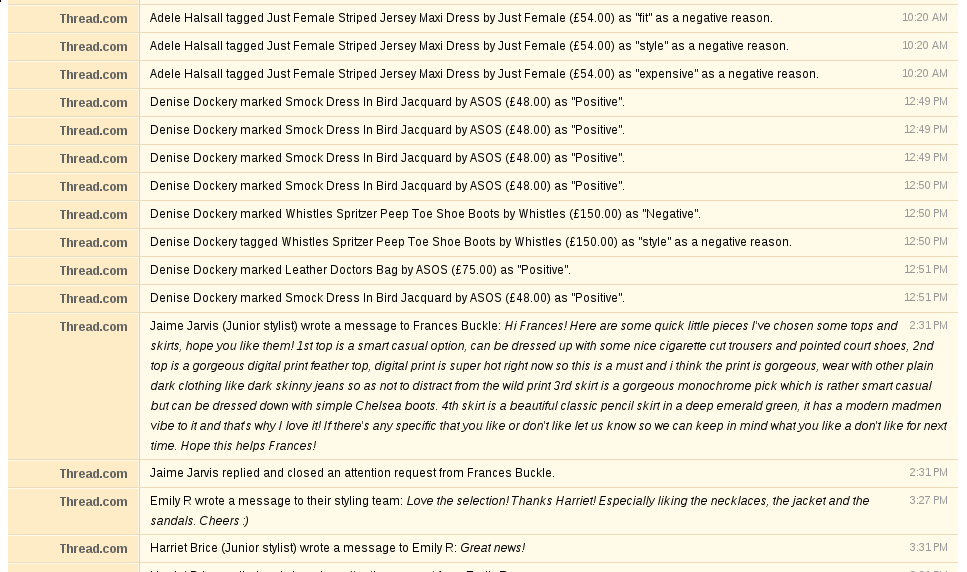
\includegraphics[width=100mm]{img/pulse.png}
}

\frame {
    \begin{itemize}
        \item For visibility, not auditing
        \item Any group chat can work. We use Hipchat.
        \item \url{https://github.com/thread/django-hipchat}
    \end{itemize}
}

\frame {
    Pulse history \\
    \vskip 1em
    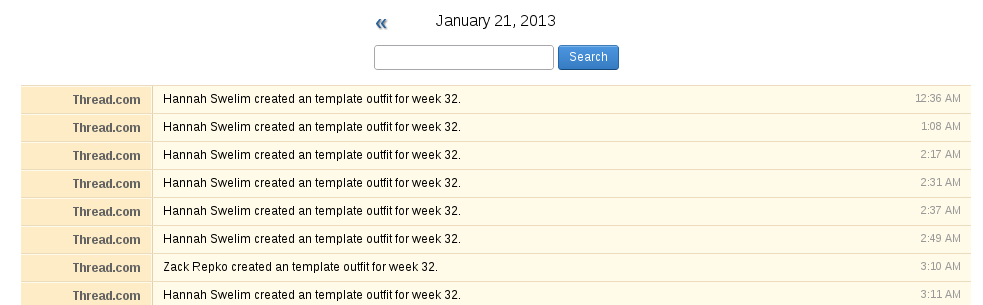
\includegraphics[width=100mm]{img/pulse-history.png}
}

\frame {
    2/4: Deploying using Debian packages
}

\frame {
    Canonical deployment (via Jenkins)

    \begin{itemize}
        \item Build .deb
        \item rsync to target hosts
        \item Install with \tt{dpkg -i}
    \end{itemize}
}

\frame {
    Example log \\
    \vskip 1em
    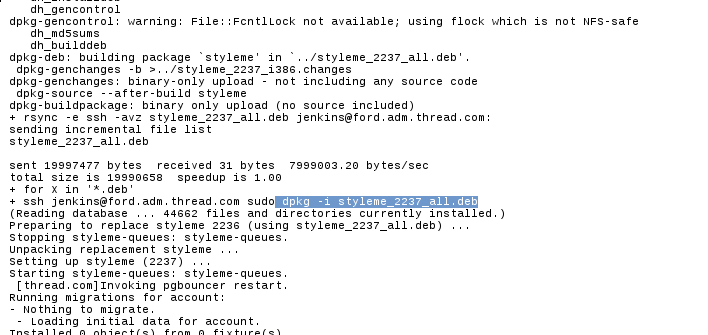
\includegraphics[width=100mm]{img/debian-deploy.png}
}

\frame {
    \tt{debian/control} \\
    \vskip 1em
    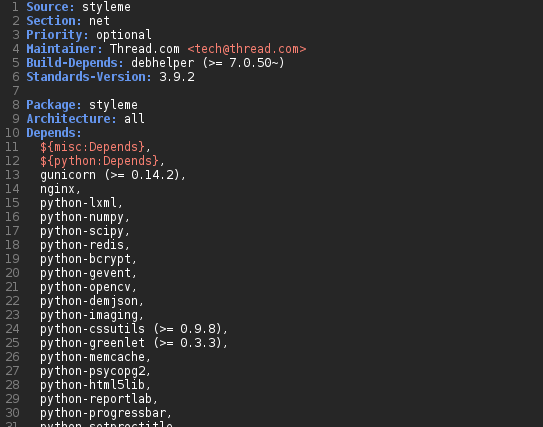
\includegraphics[width=100mm]{img/debian-control.png}
}

\frame {
    Advantages
    
    \vskip 1em

    \begin{itemize}
        \item Can happily use system packages
        \item Many tasks already done for you very well
        \item Easy to make modular system
        \item Can change a machine's purpose cleanly without reimaging
    \end{itemize}
}

\frame {
    \frametitle{Disadvantages}

    \vskip 1em

    \begin{itemize}
        \item Requires distribution-specific knowledge
        \item Inherits all Debian legacy packaging quirks
        \item Installing standalone packages with \tt{dpkg} annoying
    \end{itemize}
}

\frame {
    3/4: Auto-login links in emails
}

\frame {
    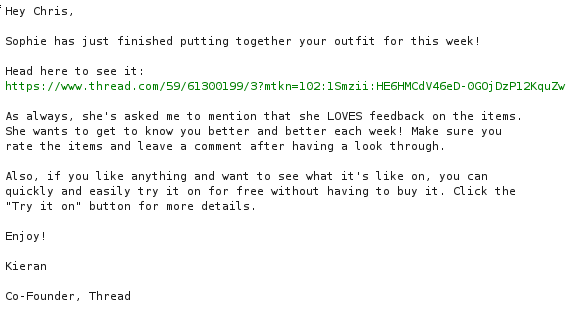
\includegraphics[width=100mm]{img/auto-login.png}
}

\frame {
    \frametitle{Our implementation}

    \begin{itemize}
        \item Allow login link to any URL simply by appending
        \item Salted HMAC implementation - no state
        \item Token includes timestamp so tokens expire
        \item Customisable salt fields - default: user.password (hashed)
        \item Tokens can be re-used (feature)
        \item \url{https://github.com/playfire/django-autologin}
    \end{itemize}
}

\frame {
    \frametitle{Recommendations}

    \begin{itemize}
        \item Salt the HMAC with the user's hashed password
        \item Include the timestamp in the hash, not the expiry time
        \item "Click here to login" copy ("The forward problem")
    \end{itemize}
}

\frame{
    \frametitle{4/4: Git HEAD version of framework}

    \begin{itemize}
        \item We run, updated approximately once a week
        \item Via an embedded code copy
    \end{itemize}
}

\frame {
    \frametitle{Advantages}

    \begin{itemize}
        \item Never complaining about missing features
        \item Increases incentive to send patches upstream
    \end{itemize}
}

\frame {
    \frametitle{Disdvantages}

    \begin{itemize}
        \item It breaks!
        \item It actually breaks other things
    \end{itemize}
}

\frame {}

\end{document}
